\section[Eric the Red]{
    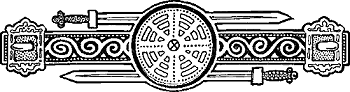
\includegraphics[width=9.3cm]{viking-tales/038}\\
    Eric the Red}

\lettrine{I}{t} was a spring day many years after Ingolf died. All the
freemen in the west of Iceland had come to a meeting. Here they made laws
and punished men for having done wrong. The meeting was over now. Men
were walking about the plain and talking. Everybody seemed much excited.
Voices were loud, arms were swinging.

``It was an unjust decision,'' some one cried. ``Eric killed the men in
fair fight. The judges outlawed him because they were afraid. His foe
Thorgest has many rich and powerful men to back him.''

``No, no!'' said another. ``Eric is a bloody man. I am glad he is out of
Iceland.''

Just then a big man with bushy red hair and beard stalked through the
crowd. He looked straight ahead and scowled.

``There he goes,'' people said, and turned to look after him.

``His hands are as red as his beard,'' some said, and frowned.

But others looked at him and smiled, saying:

``He walks like Thor the Fearless.''

``His story would make a fine song,'' one said. ``As strong and as brave
and as red as Thor! Always in a quarrel. A man of many places--Norway,
the north of Iceland, the west of Iceland, those little islands off the
shore of Iceland. Outlawed from all of them on account of his quarrels.
Where will he go now, I wonder?''

This Eric strode down to the shore with his men following.

``He is in a black temper,'' they said. ``We should best not talk to
him.''

So they made ready the boat in silence. Eric got into the pilot's seat
and they sailed off. Soon they pulled the ship up on their own shore.
Eric strolled into his house and called for supper. When the
drinking-horns had been filled and emptied, Eric pulled himself up and
smiled and shouted out so that the great room was full of his big voice:

``There is no friend like mead. It always cheers a man's heart.''

\begin{figure}
    \centering
    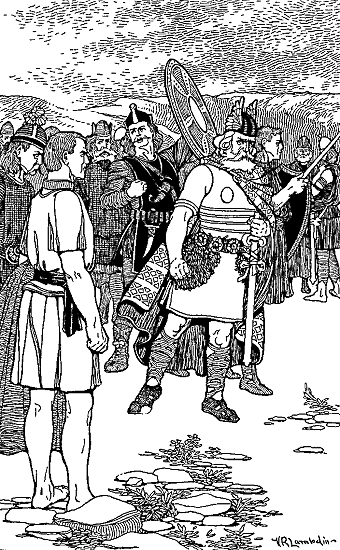
\includegraphics[width=9.1cm]{viking-tales/039}
    \caption{``He looked straight ahead of him and scowled''}
\end{figure}

Then laughter and talking began in the hall because Eric's good temper
had come back. After a while Eric said:

``Well, I must off somewhere. I have been driven about from place to
place, like a seabird in a storm. And there is always a storm about me.
It is my sword's fault. She is ever itching to break her
peace-bands\footnote{See note about peace-bands on
page~\pageref{peace-bands}.} and be out and at the play. She has shut
Norway to me and now Iceland. Where will you go next, old comrade?'' and
he pulled out his sword and looked at it and smiled as the fire flashed
on it.

``There are some of us who will follow you wherever you go, Eric,''
called a man from across the fire.

``Is it so?'' Eric cried, leaping up. ``Oh! then we shall have some
merry times yet. Who will go with me?''

More than half the men in the hall jumped to their feet and waved their
drinking-horns and shouted:

``I! I!''

\begin{figure}
    \centering
    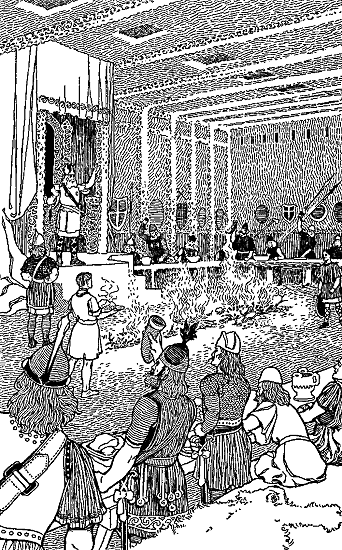
\includegraphics[width=9.1cm]{viking-tales/040}
    \caption{``ore than half the men in the hall jumped to their feet''}
\end{figure}

Eric sat down in his chair and laughed.

``O you bloody birds of battle!'' he cried. ``Ever hungry for new
frolic! Our swords are sisters in blood, and we are brothers in
adventure. Do you know what is in my heart to do?''

He jumped to his feet, and his face glowed. Then he laughed as he looked
at his men.

``I see the answer flashing from your eyes,'' he said, ``that you will
do it even if it is to go down to Niflheim and drag up Hela, the pale
queen of the stiff dead.''

His men pounded on the tables and shouted:

``Yes! Yes! Anywhere behind Eric!''

``But it is not to Niflheim,'' Eric laughed. ``Did you ever hear that
story that Gunnbiorn told? He was sailing for Iceland, but the fog came
down, and then the wind caught him and blew him far off. While he
drifted about he saw a strange land that rose up white and shining out
of a blue sea. Huge ships of ice sailed out from it and met him. I mean
to sail to that land.''

A great shout went up that shook the rafters. Then the men sat and
talked over plans. While they sat, a stranger came into the hall.

``I have no time to drink,'' he said. ``I have a message from your
friend Eyjolf. He says that Thorgest with all his men means to come here
and catch you to-night. Eyjolf bids you come to him, and he will hide
you until you are ready to start; for he loves you.''

``Hunted like a wolf from corner to corner of the world!'' Eric cried
angrily. ``Will they not even let me finish one feast?''

Then he laughed.

``But if I take my sport like a wolf, I must be hunted like one. So we
shall sleep to-night in the woods about Eyjolf's house, comrades,
instead of in these good beds. Well, we have done it before.''

``And it is no bad place,'' cried some of the men.

``I always liked the stars better than a smoky house fire,'' said one.

``Can no bad fortune spoil your good nature?'' laughed Eric. ``But now
we are off. Let every man carry what he can.''

So they quickly loaded themselves with clothes and gold and swords and
spears and kettles of food. Eric led his wife Thorhild and his two young
sons, Thorstein and Leif. All together they got into the boat and went
to Eyjolf's farm. For a week or more they stayed in his woods, sometimes
in a secret cave of his when they knew that Thorgest was about. And
sometimes Eyjolf sent and said:

``Thorgest is off. Come to my house for a feast.''

All this time they were making ready for the voyage, repairing the ship
and filling it with stores. Word of what Eric meant to do got out, and
men laughed and said:

``Is that not like Eric? What will he not do?''

Some men liked the sound of it, and they came to Eric and said:

``We will go with you to this strange land.''

So all were ready and they pushed off with Eric's family aboard and
those friends who had joined him. They took horses and cattle with them,
and all kinds of tools and food.

``I do not well know where this land is,'' Eric said. ``Gunnbiorn said
only that he sailed east when he came home to Iceland. So I will steer
straight west. We shall surely find something. I do not know, either,
how long we must go.''

So they sailed that strange ocean, never dreaming what might be ahead of
them. They found no islands to rest on. They met heavy fogs.

One day as Eric sat in the pilot's seat, he said:

``I think that I see one of Gunnbiorn's ships of ice. Shall we sail up
to her and see what kind of a craft she is?''

``Yes,'' shouted his men.

So they went on toward it.

``It sends out a cold breath,'' said one of the men.

They all wrapped their cloaks about them.

``It is a bigger boat than I ever saw before,'' said Eric. ``The white
mast stands as high as a hill.''

``It must be giants that sail in it, frost giants,'' said another of the
men.

But as they came nearer, Eric all at once laughed loudly and called out:

``By Thor, that Gunnbiorn was a foolish fellow. Why, look! It is only a
piece of floating ice such as we sometimes see from Iceland. It is no
ship, and there is no one on it.''

His men laughed and one called to another and said:

``And you thought of frost giants!''

Then they sailed on for days and days. They met many of these icebergs.
On one of them was a white bear.

``Yonder is a strange pilot,'' Eric laughed.

``I have seen bears come floating so to the north shore of Iceland,'' an
old man said. ``Perhaps they come from the land that we are going to
find.''

One day Eric said:

``I see afar off an iceberg larger than any one yet. Perhaps that is our
white land.''

\begin{figure}
    \centering
    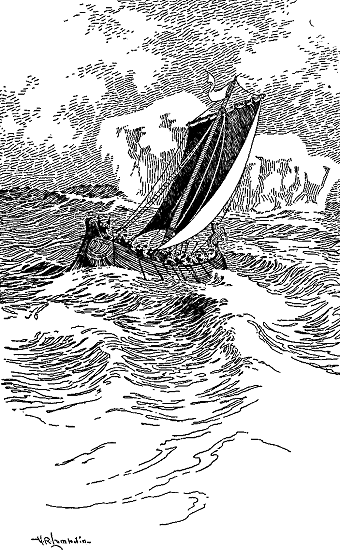
\includegraphics[width=9.1cm]{viking-tales/041}
    \caption{``It is a bigger boat than I ever saw before''}
\end{figure}

But even as he said it he felt his boat swing under his hand as he held
the tiller. He bore hard on the rudder, but he could not turn the ship.

``What is this?'' he cried. ``A strong river is running here. It is
carrying our ship away from this land. I cannot make head against it.
Out with the oars!''

So with oars and sail and rudder they fought against the current, but it
took the boat along like a chip, and after a while they put up their
oars and drifted.

``Luck has taken us into its own hands,'' Eric laughed. ``But this is as
good a way as another.''

Sometimes they were near enough to see the land, then they were carried
out into the sea and thought that they should never see any land again.

``Perhaps this river will carry us to a whirlpool and suck us under,''
the men said.

But at last Eric felt the current less strong under his hand.

``To the oars again!'' he called.

So they fought with the current and sailed out of it and went on toward
land. But when they reached the shore they found no place to go in.
Steep black walls shot up from the sea. Nothing grew on them. When the
men looked above the cliffs they saw a long line of white cutting the
sky.

``It is a land of ice,'' they said.

They sailed on south, all the time looking for a place to go ashore.

``I am sick of this endless sea,'' Thorhild complained, ``but this land
is worse.''

After a while they began to see small bays cut into the shore with
little flat patches of green at their sides. They landed in these places
and stretched and warmed themselves and ate.

``But these spots are only big enough for graves,'' the men said. ``We
can not live here.''

So they went on again. All the time the weather was growing colder.
Eric's people kept themselves wrapped in their cloaks and put scarfs
around their heads.

``And it is still summer!'' Thorhild said. ``What will it be in
winter?''

``We must find a place to build a house now before the winter comes
on,'' said Eric. ``We must not freeze here.''

So they chose a little spot with hills about it to keep off the wind.
They made a house out of stones; for there were many in that place. They
lived there that winter. The sea for a long way out from shore froze so
that it looked like white land. The men went out upon it to hunt white
bear and seal. They ate the meat and wore the skins to keep them warm.
The hardest thing was to get fuel for the fire. No trees grew there. The
men found a little driftwood along the shore, but it was not enough. So
they burned the bones and the fat of the animals they killed.

``It is a sickening smell,'' Thorhild said. ``I have not been out of
this mean house for weeks. I am tired of the darkness and the smoke and
the cattle. And all the time I hear great noises, as though some giant
were breaking this land into pieces.''

``Ah, cheer up, good wife!'' Eric laughed. ``I smell better luck
ahead.''

Once Eric and his men climbed the cliffs and went back into the middle
of the land. When they came home they had this to tell:

``It is a country of ice, shining white. Nothing grows on it but a few
mosses. Far off it looks flat, but when you walk upon it, there are
great holes and cracks. We could see nothing beyond. There seems to be
only a fringe of land around the edge of an island of ice.''

The winter nights were very long. Sometimes the sun showed for an hour,
sometimes for only a few minutes, sometimes it did not show at all for a
week. The men hunted by the bright shining of the moon or by the
northern lights.

As it grew warmer the ice in the sea began to crack and move and melt
and float away. Eric waited only until there was a clear passage in the
water. Then he launched his boat, and they sailed southward again. At
last they found a place that Eric liked.

``Here I will build my house,'' he said.

So they did and lived there that summer and pastured their cattle and
cut hay for the winter and fished and hunted.

The next spring Eric said:

``The land stretches far north. I am hungry to know what is there.''

Then they all got into the boat again and sailed north.

``We can leave no one here,'' Eric had said. ``We cannot tell what might
come between us. Perhaps giants or dragons or strange men might come out
of this inland ice and kill our people. We must stay together.''

Farther north they found only the same bare, frozen country. So after a
while they sailed back to their home and lived there.

One spring after they had been in that land for four years, Eric said:

``My eyes are hungry for the sight of men and green fields again. My
stomach is sick of seal and whale and bear. My throat is dry for mead.
This is a bare and cold and hungry land. I will visit my friends in
Iceland.''

``And our swords are rusty with long resting,'' said his men. ``Perhaps
we can find play for them in Iceland.''

``Now I have a plan,'' Eric suddenly said. ``Would it not be pleasant to
see other feast halls as we sail along the coast?''

``Oh! it would be a beautiful sight,'' his men said.

``Well,'' said Eric, ``I am going to try to bring back some neighbors
from Iceland. Now we must have a name for our land. How does Greenland
sound?''

His men laughed and said:

``It is a very white Greenland, but men will like the sound of it. It is
better than Iceland.''

So Eric and all his people sailed back and spent the winter with his
friends.

``Ah! Eric, it is good to hear your laugh again,'' they said.

Eric was at many feasts and saw many men, and he talked much of his
Greenland.

``The sea is full of whale and seals and great fish,'' he said. ``The
land has bear and reindeer. There are no men there. Come back with me
and choose your land.''

Many men said that they would do it. Some men went because they thought
it would be a great frolic to go to a new country. Some went because
they were poor in Iceland and thought:

``I can be no worse off in Greenland, and perhaps I shall grow rich
there.''

And some went because they loved Eric and wanted to be his neighbors.

So the next summer thirty-five ships full of men and women and goods
followed Eric for Greenland. But they met heavy storms, and some ships
were wrecked, and the men drowned. Other men grew heartsick at the
terrible storm and the long voyage and no sight of land, and they turned
back to Iceland. So of those thirty-five ships only fifteen got to
Greenland.

``Only the bravest and the luckiest men come here,'' Eric said. ``We
shall have good neighbors.''

Soon other houses were built along the fiords.

``It is pleasant to sail along the coast now,'' said Eric. ``I see smoke
rising from houses and ships standing on the shore and friendly hands
waving.''
